\clearpage
\section{Implementation Details}

\subsection{The details of your model (MultiHeadAttention)}
This is a model detail section.
\begin{lstlisting}[language=Python, caption=Multi-Head Attention 實作]
class MultiHeadAttention(nn.Module):
    def __init__(self, dim=768, num_heads=16, attn_drop=0.1):
        super(MultiHeadAttention, self).__init__()
        self.num_heads = num_heads
        self.dim = dim
        self.head_dim = dim // num_heads # 768//16 = 48
        self.qkv = nn.Linear(dim, dim * 3)
        self.proj = nn.Linear(dim, dim)
        self.attn_drop = nn.Dropout(attn_drop)
        self.scale = self.head_dim ** -0.5

    def forward(self, x):
        batch_size, num_image_tokens, dim = x.shape
        qkv = self.qkv(x)
        qkv = qkv.reshape(batch_size, num_image_tokens, 3, self.num_heads, self.head_dim)
        q, k, v = qkv.permute(2, 0, 3, 1, 4)
        attn = (q @ k.transpose(-2, -1)) * self.scale 
        attn = attn.softmax(dim=-1)
        attn = self.attn_drop(attn)
        x = (attn @ v).transpose(1, 2).reshape(batch_size, num_image_tokens, dim)
        x = self.proj(x)
        return x
\end{lstlisting}


\subsection{The details of your stage2 training (Masked Generative Image Transformer)}
This is a stage2 training detail section.

\subsubsection{Learning rate strategy}
This is a section of learning strategy.





\subsubsection{Information flow of Masked Generative Image Transformer}
This is a section of information flow of Masked Generative Image Transformer.

\subsubsection{Dynamic Masking Ratio when training}
This is a section of dynamic masking ratio when training.

\subsection{The details of your inference for inpainting task (using Masked Generative Image Transformer)}
This is an inference detail section. 

\subsubsection{Gamma strategy}
This is a section of gamma strategy.

我想要測試當 MaskGIT 大膽的生成 token 之後,在拔掉一些信心不高的 token 這個策略會不會讓 FID score 更低。

\begin{figure}[h]
    \centering
    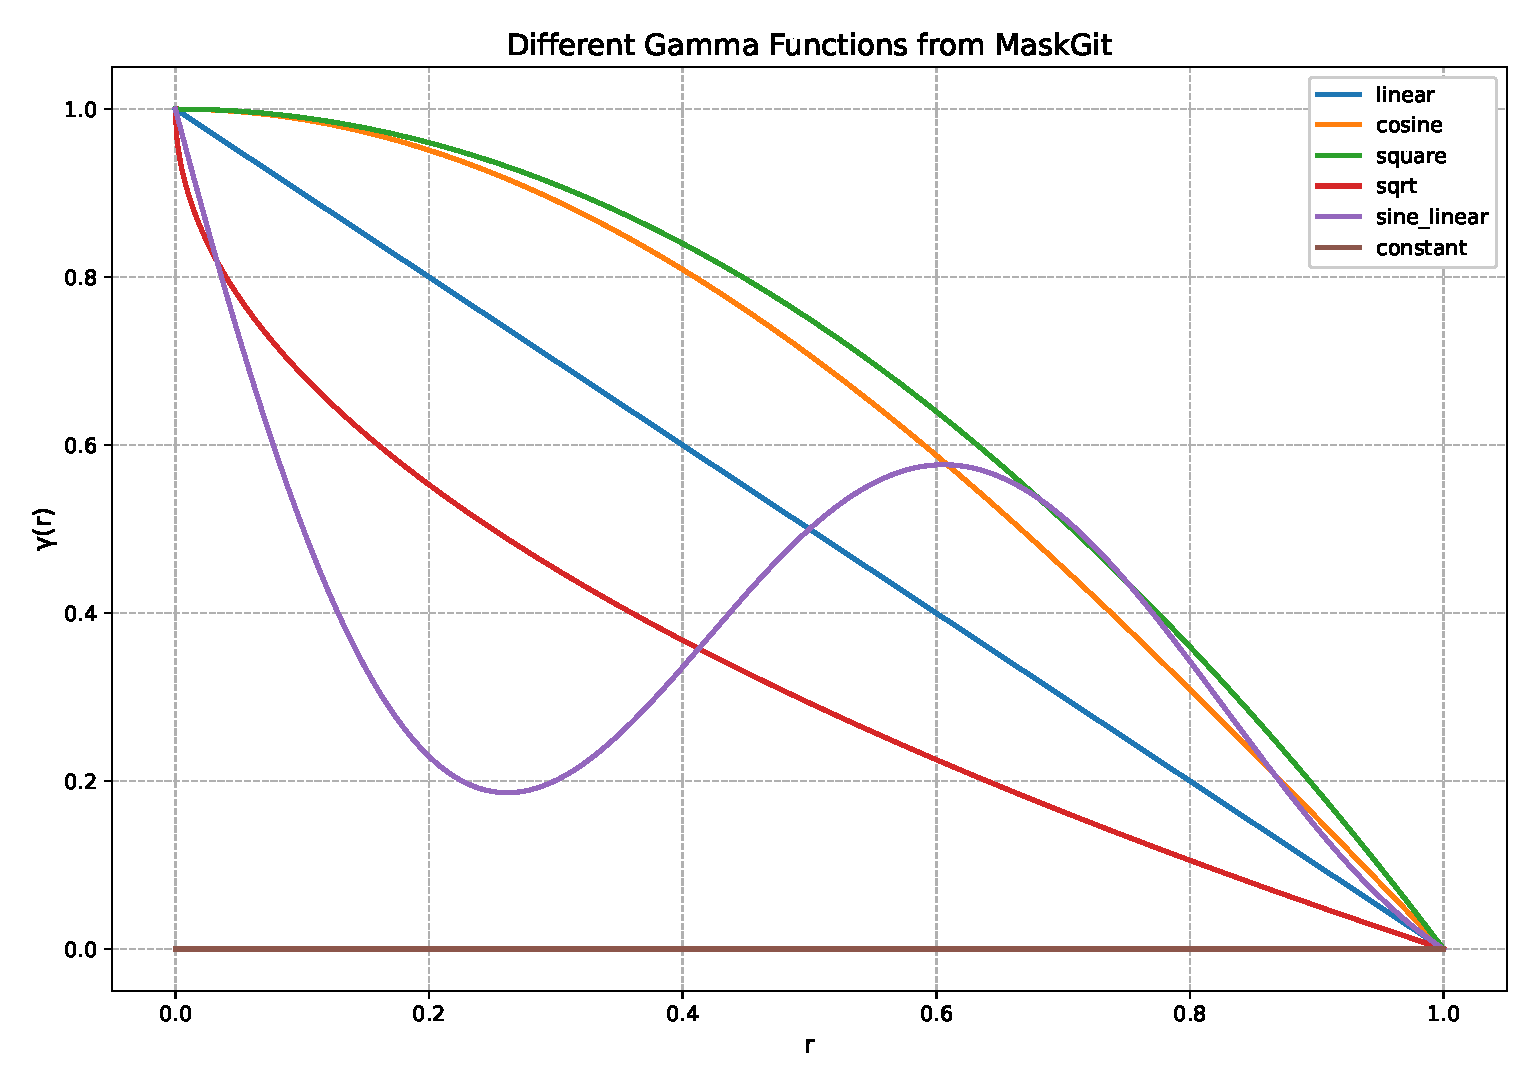
\includegraphics[width=\textwidth]{figures/gamma_functions}
    \caption{不同的 gamma 函數策略}
    \label{fig:gamma_functions}
\end{figure}

我們使用以下的數學式來設計 sine linear gamma 函數:

\begin{equation}
    \gamma(r) = (1-r)(1-0.75\sin(2\pi r))
\end{equation}

其中 $r$ 是目前生成的比例 (0 到 1 之間)。這個函數有以下特性:

\begin{itemize}
    \item 當 $r=0$ 時, $\gamma(0)=1$, 代表一開始要生成所有 token
    \item 當 $r=1$ 時, $\gamma(1)=0$, 代表最後所有 token 都要確定
    \item $\sin(2\pi r)$ 項讓函數在生成過程中有大膽生成 token 的階段以及,移除信心不高的 token 的階段。
    \item 0.75 係數控制波動的幅度
    \item $(1-r)$ 項確保整體遞減趨勢
\end{itemize}

